\chapter[Search for the decays $\Bp\!\to hhh\mumu$]{Search for the decays $\boldsymbol{\Bp\!\to hhh\mumu}$}
\label{ch:hhh}

cats



%\section{Motivation}
%Chapter~\ref{ch:theory} describes the importance of FCNCs and the precise measurements of processes
%involving loops since they are sensitive to new physics at energy scales far above that which the
%interaction has direct access to.
%One such FCNC transistion is that of \decay{b}{s\ell^+\ell^-}, which has the CKM matrix elements
%\V{tb} and \V{ts} in the leading order diagram.
%The lepton pair is a product of a decaying $Z$ or $\gamma$, by lepton universality all leptons are
%equally likely, however \lhcb is particularly adept at muon identification.

%The \lhcb collaboration has published many interesting results with the \decay{b}{s\mumu} FCNC, not
%least the first observation of \decay{\Bs}{\mumu}.
%There is also much interest surrounding the \decay{\Bd}{\Kstar\mumu}, which is a \decay{b}{s} FCNC
%transisiton with a spectator quark, and then the decay of the \Kstar.
%An analagous diagram is also possible, but instead of the \Kstar the final state is \kpipi.
%This has additional interest in that, not only does it probe the FCNC, but the \kpipi system can
%result from the decay of numerous strange resonances.
%These resonances have been previously studied in the decay \btojpsikpipi by the \belle
%collaboration.

%The principal decay mode that results in the $\kpipi\mumu$ final state is
%\decay{\Bp}{K_1(1270)^+\mumu}, where \decay{K_1(1270)}{\kpipi}.
%The \kone:

%The composition of the $\Kp\pip\pim$ spectrum of the decay $\Bp\to\jpsi\Kp\pip\pim$ has been
%previously studied in Ref.~\cite{Guler:2010if}.
%For the decay $\Bp\to\Kp\pip\pim\mup\mun$ the final state is expected to be dominated by
%contributions from the $K_1(1270)^+$ and $K_1(1400)^+$ resonances.
%The mass eigenstates $K_1(1270)^+$ and $K_1(1400)^+$ are a mixture of the $1^3P_1$ and $1^1P_1$
%states according to
%\begin{align}
  %\ket{K_1(1270)} &= \ket{K(1^3P_1)}\sin\theta_{K_1} + \ket{K(1^1P_1)}\cos\theta_K,\nonumber\\
  %\ket{K_1(1400)} &= \ket{K(1^3P_1)}\cos\theta_{K_1} - \ket{K(1^1P_1)}\sin\theta_K,%\\
  %\label{eq:k1mixing}
%\end{align}
%where $\theta_K$ denotes the $1^3P_1\text{--}1^1P_1$ %$K_1(1270)^+\text{--}K_1(1400)^+$
%mixing angle~\cite{Hatanaka:2008gu}.








%Again, look at the ANA and PAPER.
%
%\begin{figure}
  %\begin{center}
    %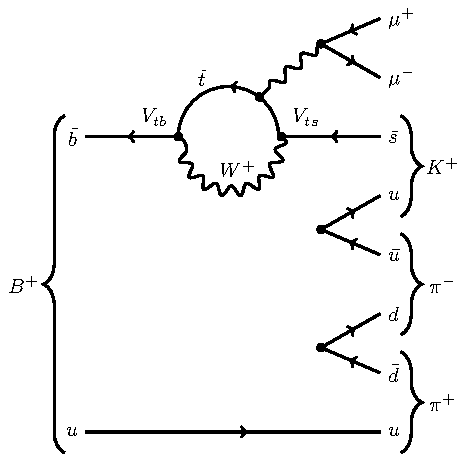
\includegraphics[scale=1]{feynman_hhh_kpipimumu}
    %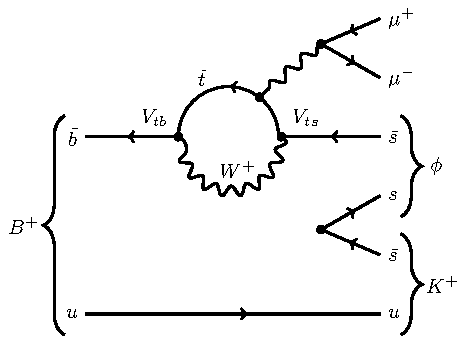
\includegraphics[scale=1]{feynman_hhh_phikmumu}
  %\end{center}
  %\caption[Feynman diagrams for \btokpipimumu and \btophikmumu]
  %{\small
  %Feynman diagrams for $hhh$
%}
%\end{figure}
%
%\section{Motivation}
%\section{Theory specific to these channels}
%\begin{itemize}
  %\item $\theta K_1$ mixing angle
  %\item Strange resonances
%\end{itemize}
%\section{Data sample}
%\section{Selection}
%\section{Results}
%
%\begin{figure}
  %\begin{center}
    %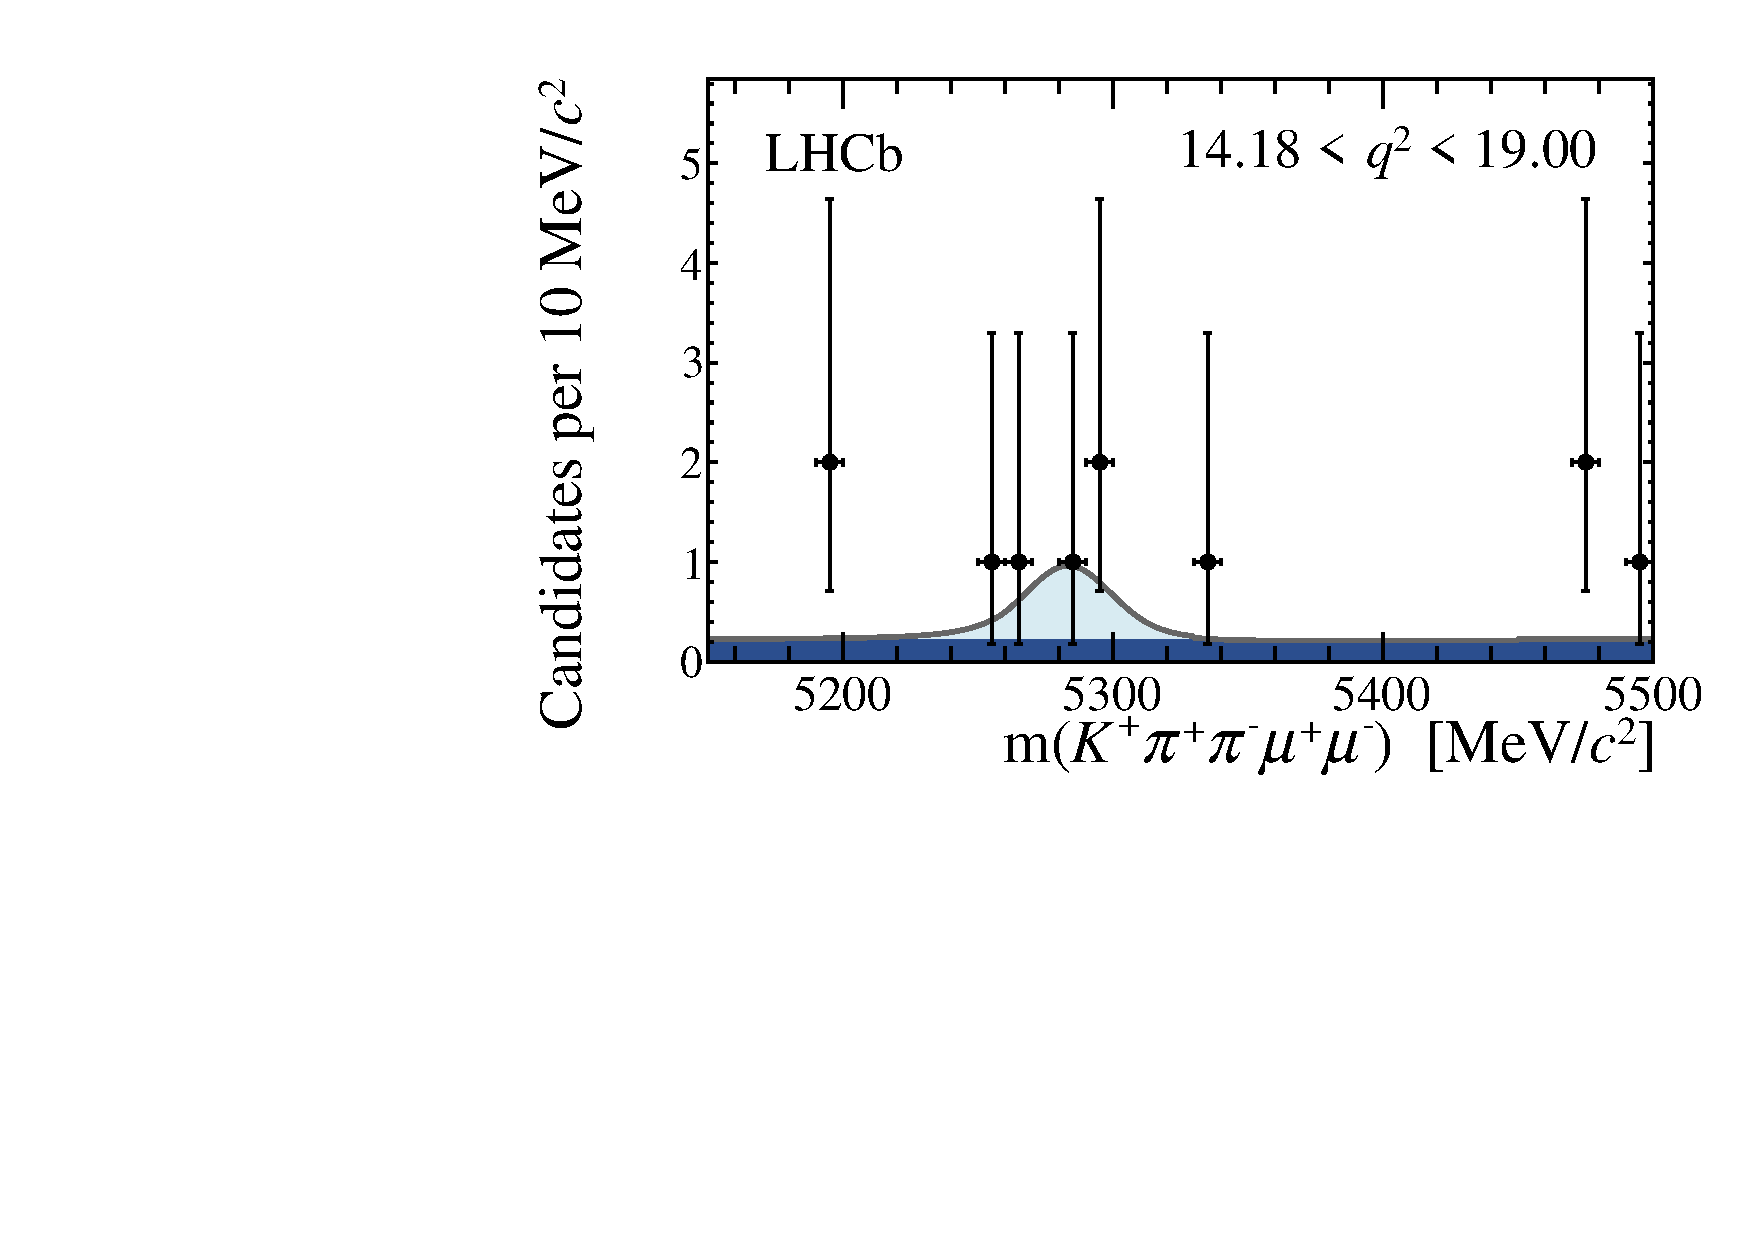
\includegraphics[width=0.48\textwidth]{q2_r6}
    %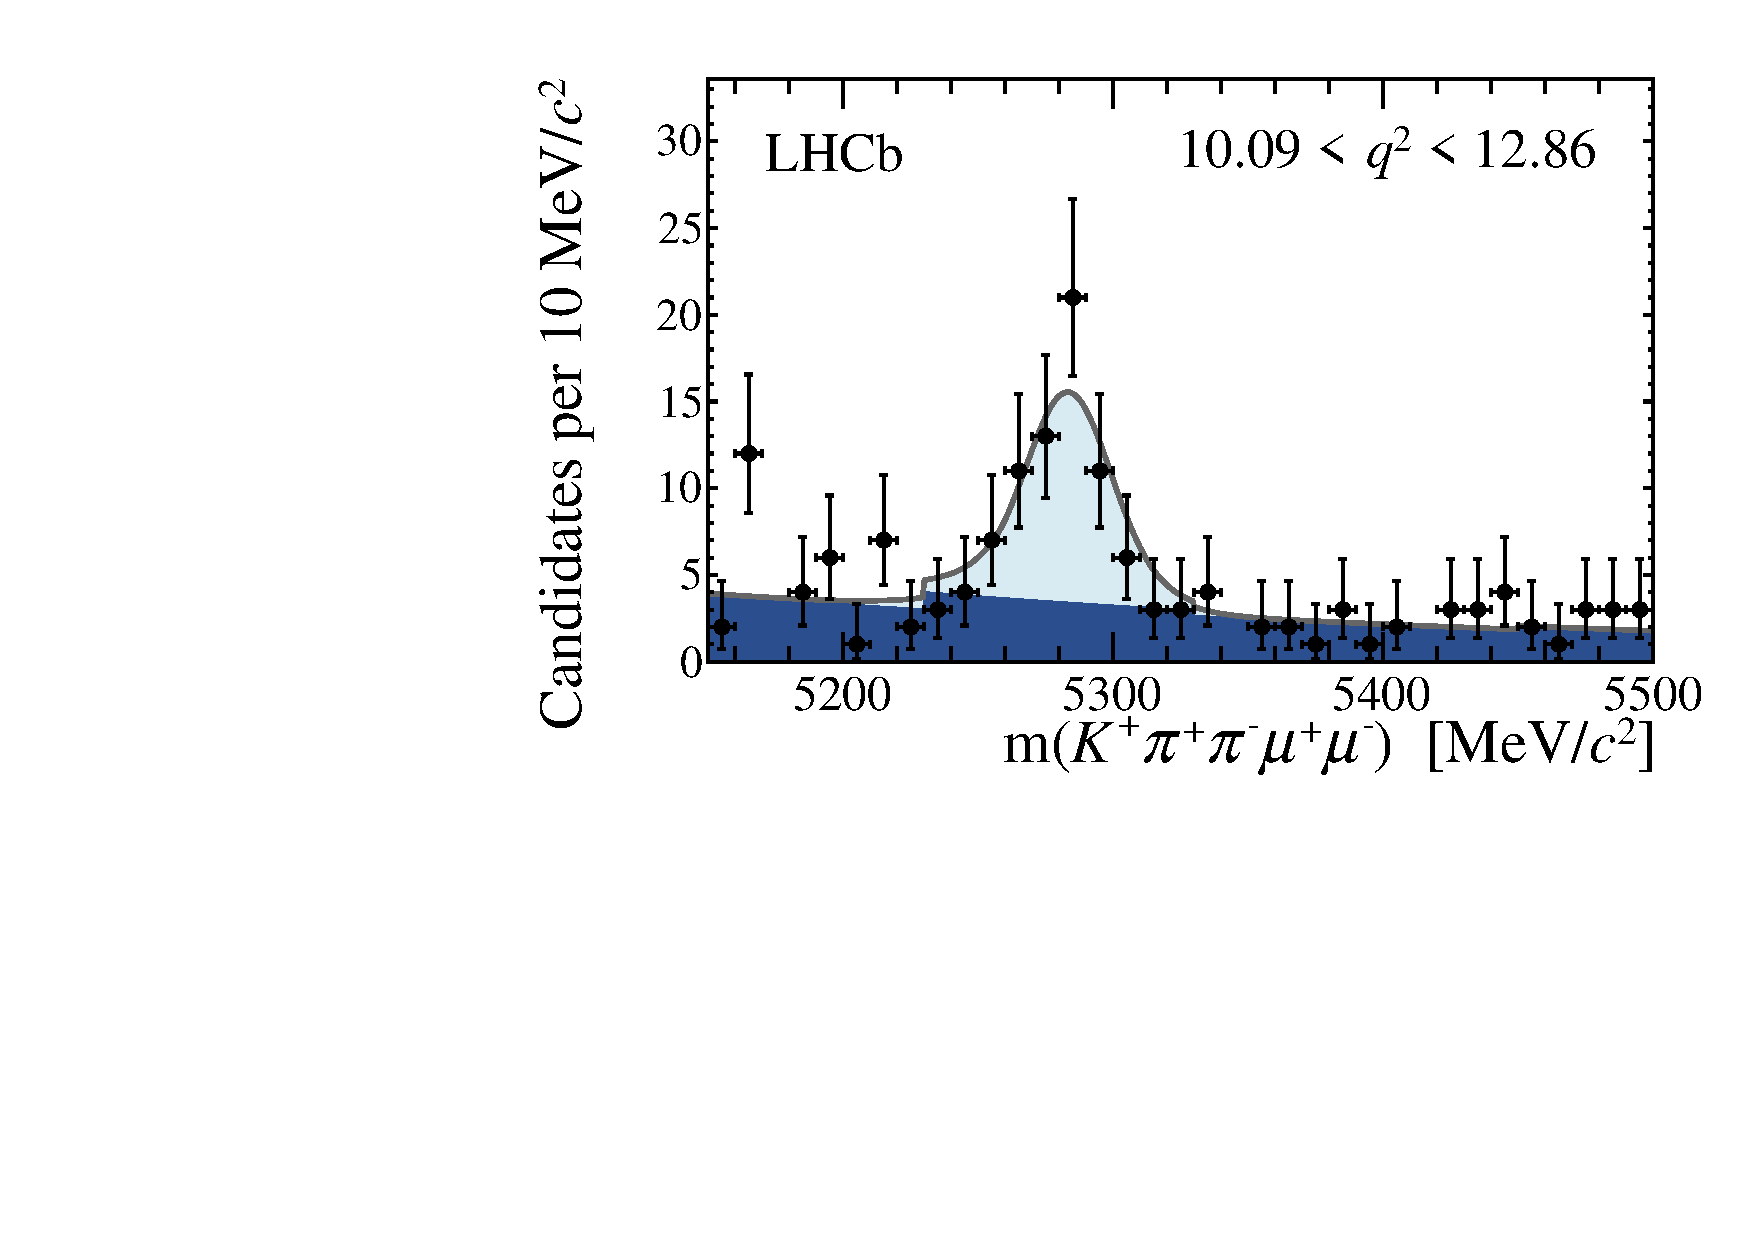
\includegraphics[width=0.48\textwidth]{q2_r5}
    %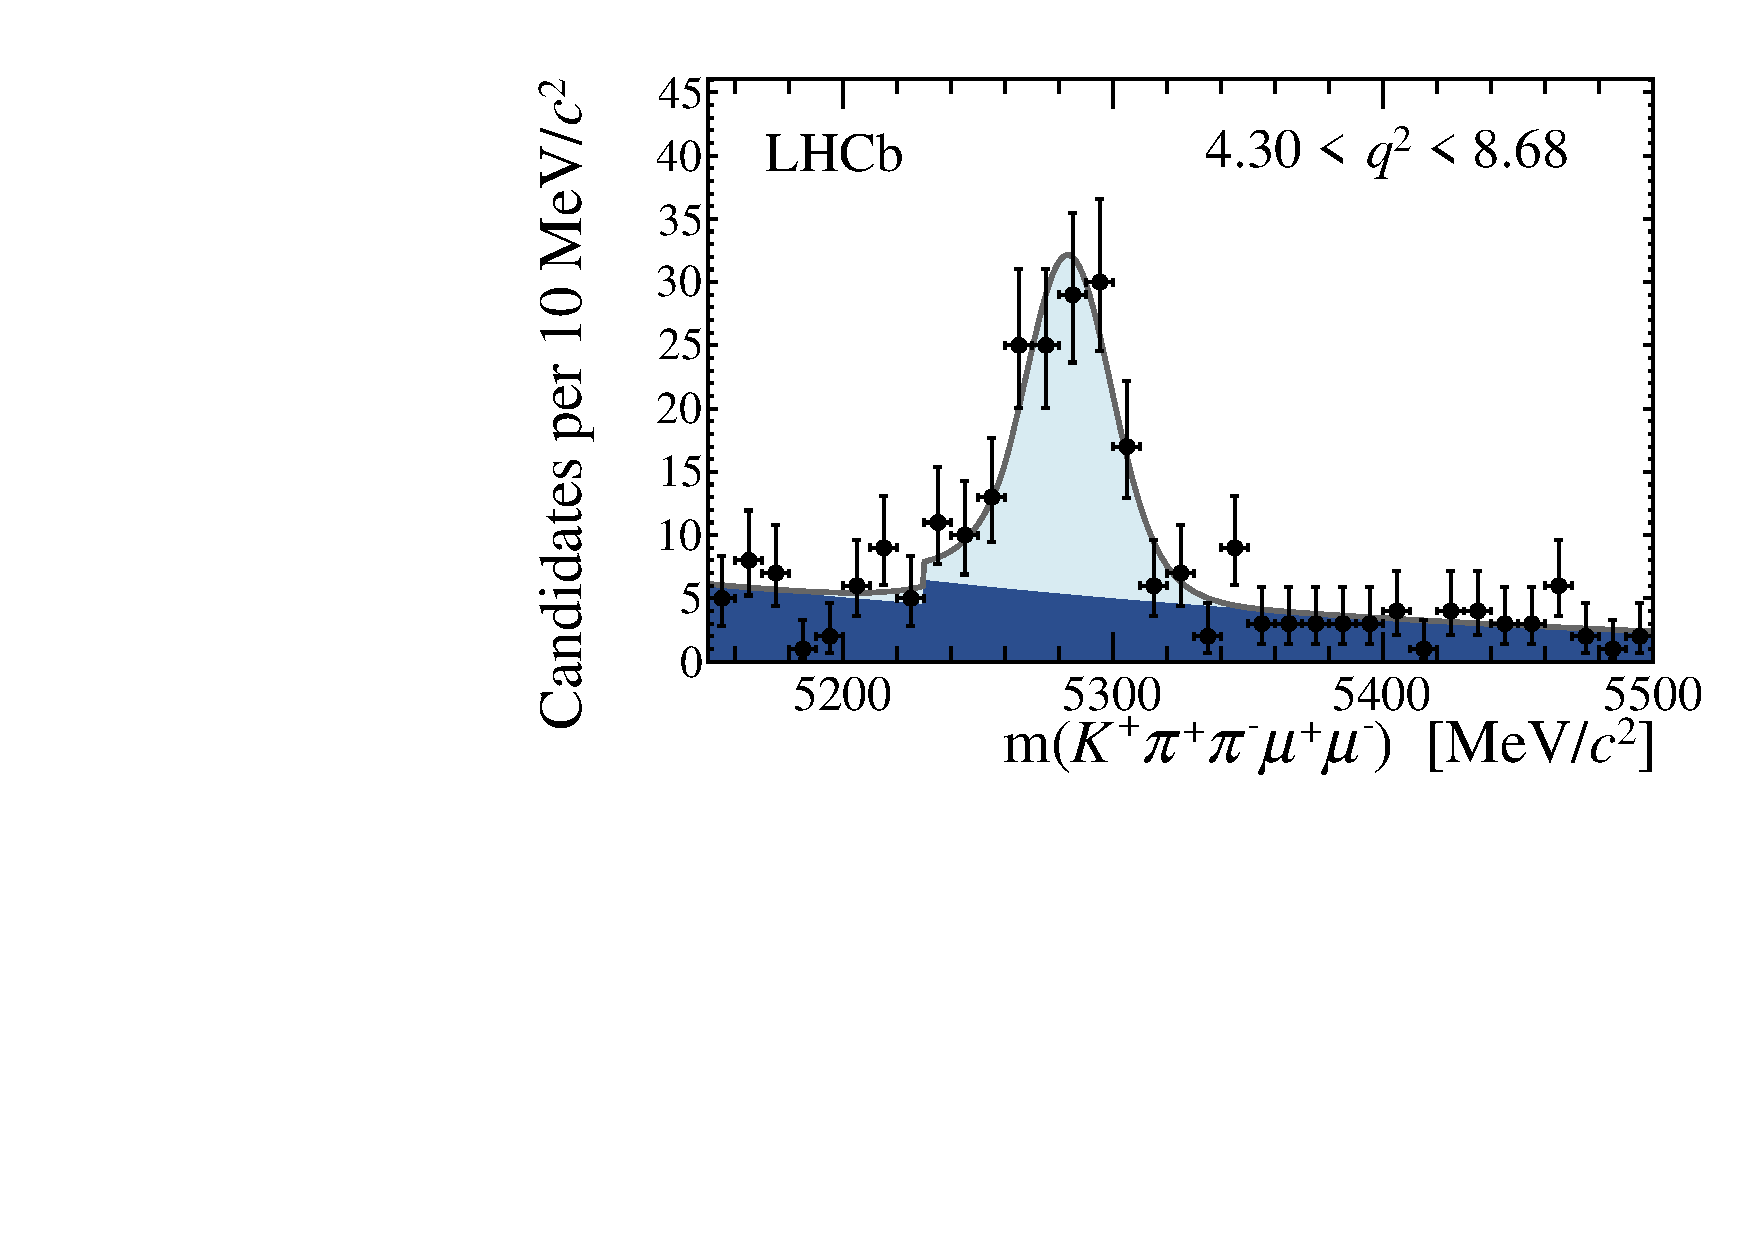
\includegraphics[width=0.48\textwidth]{q2_r4}
    %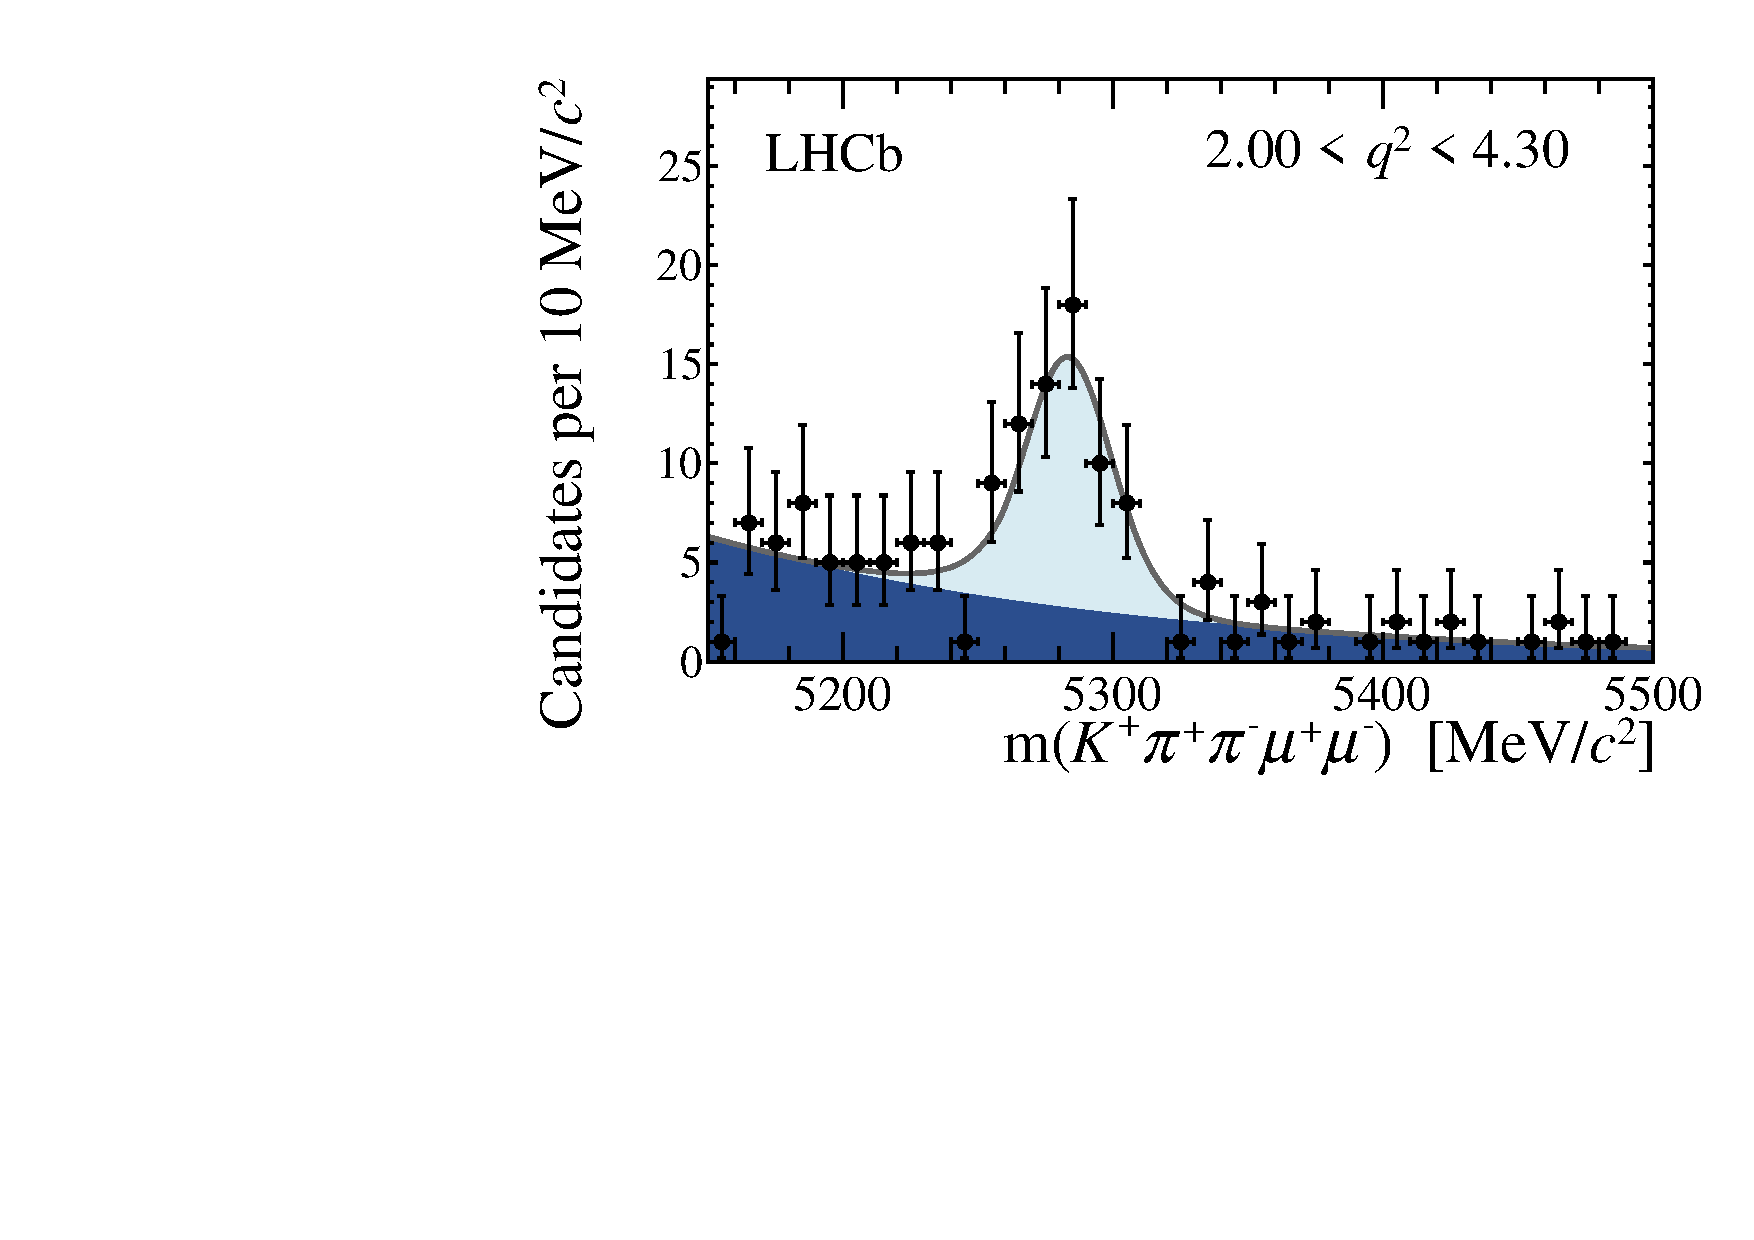
\includegraphics[width=0.48\textwidth]{q2_r3}
    %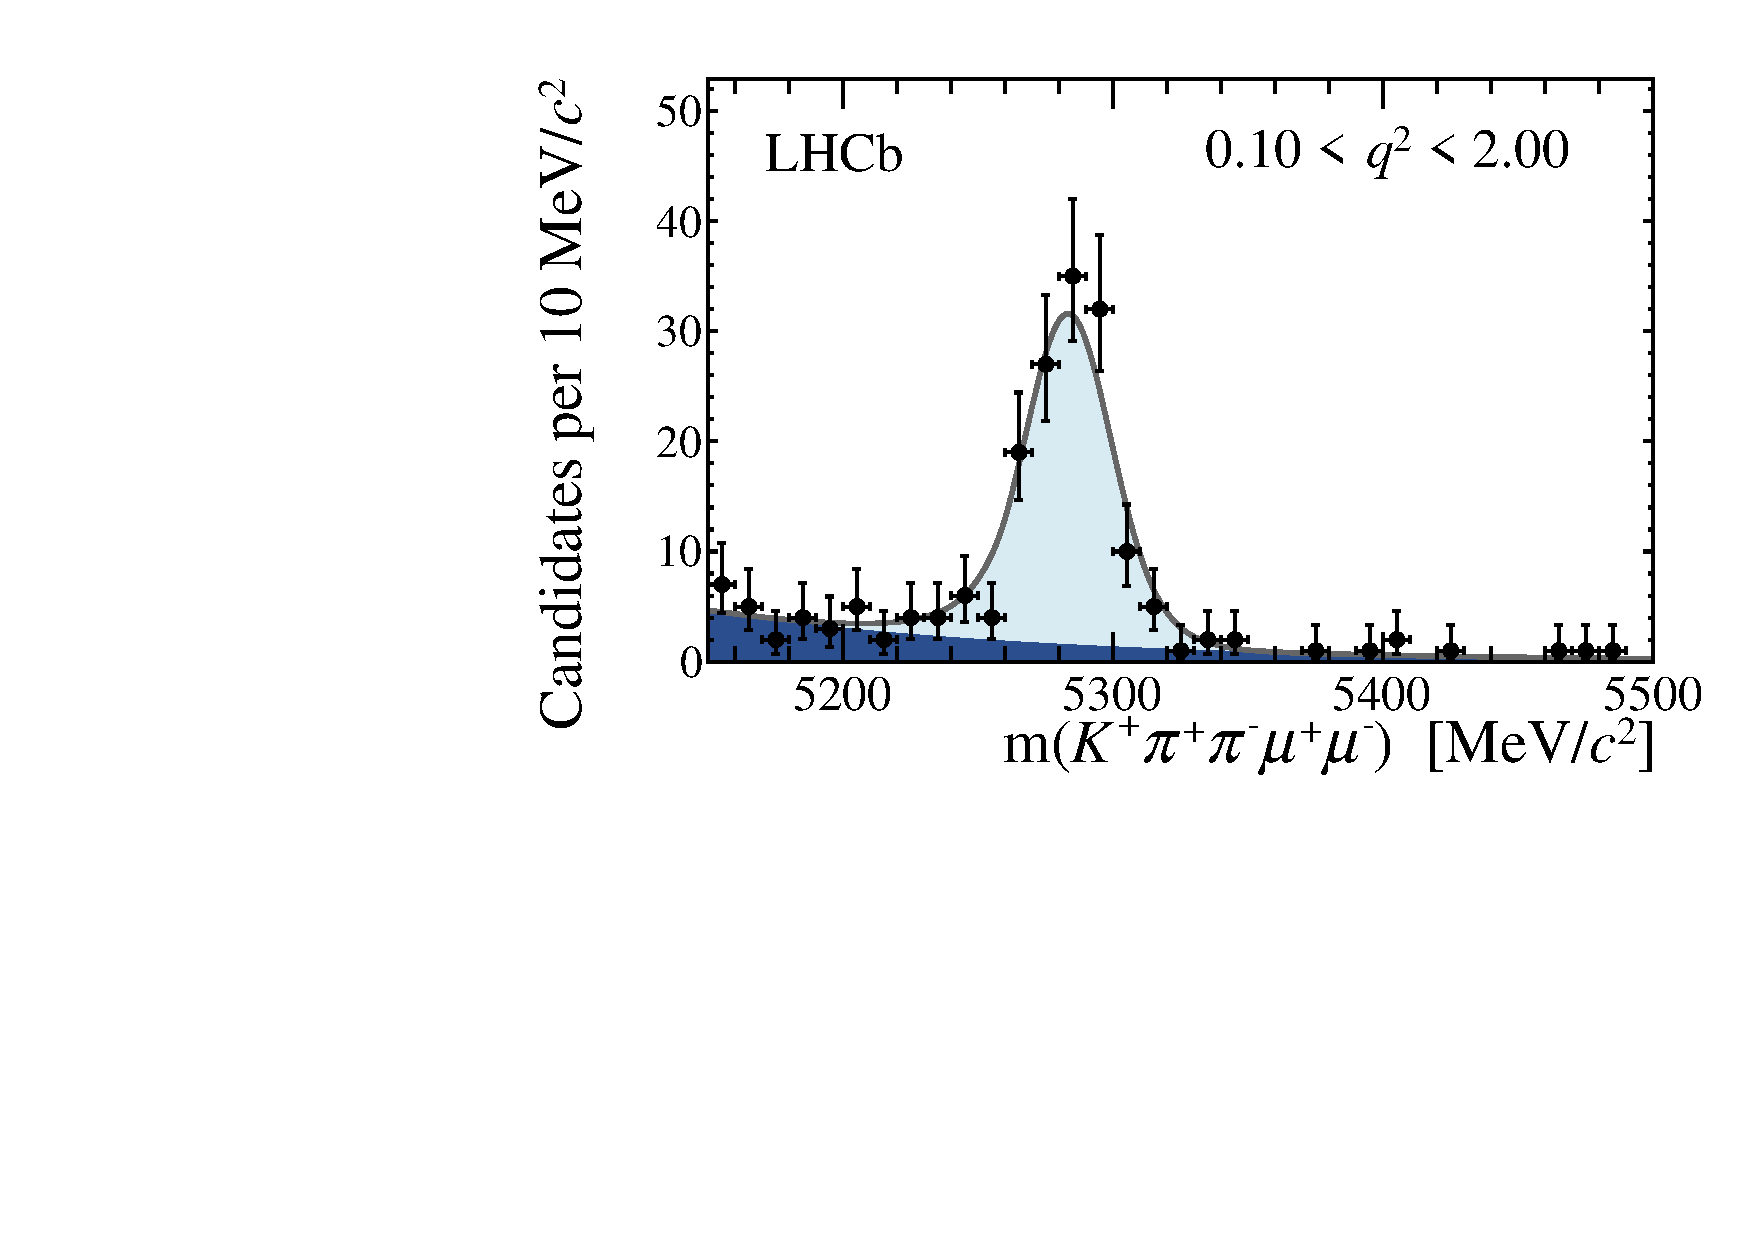
\includegraphics[width=0.48\textwidth]{q2_r2}
    %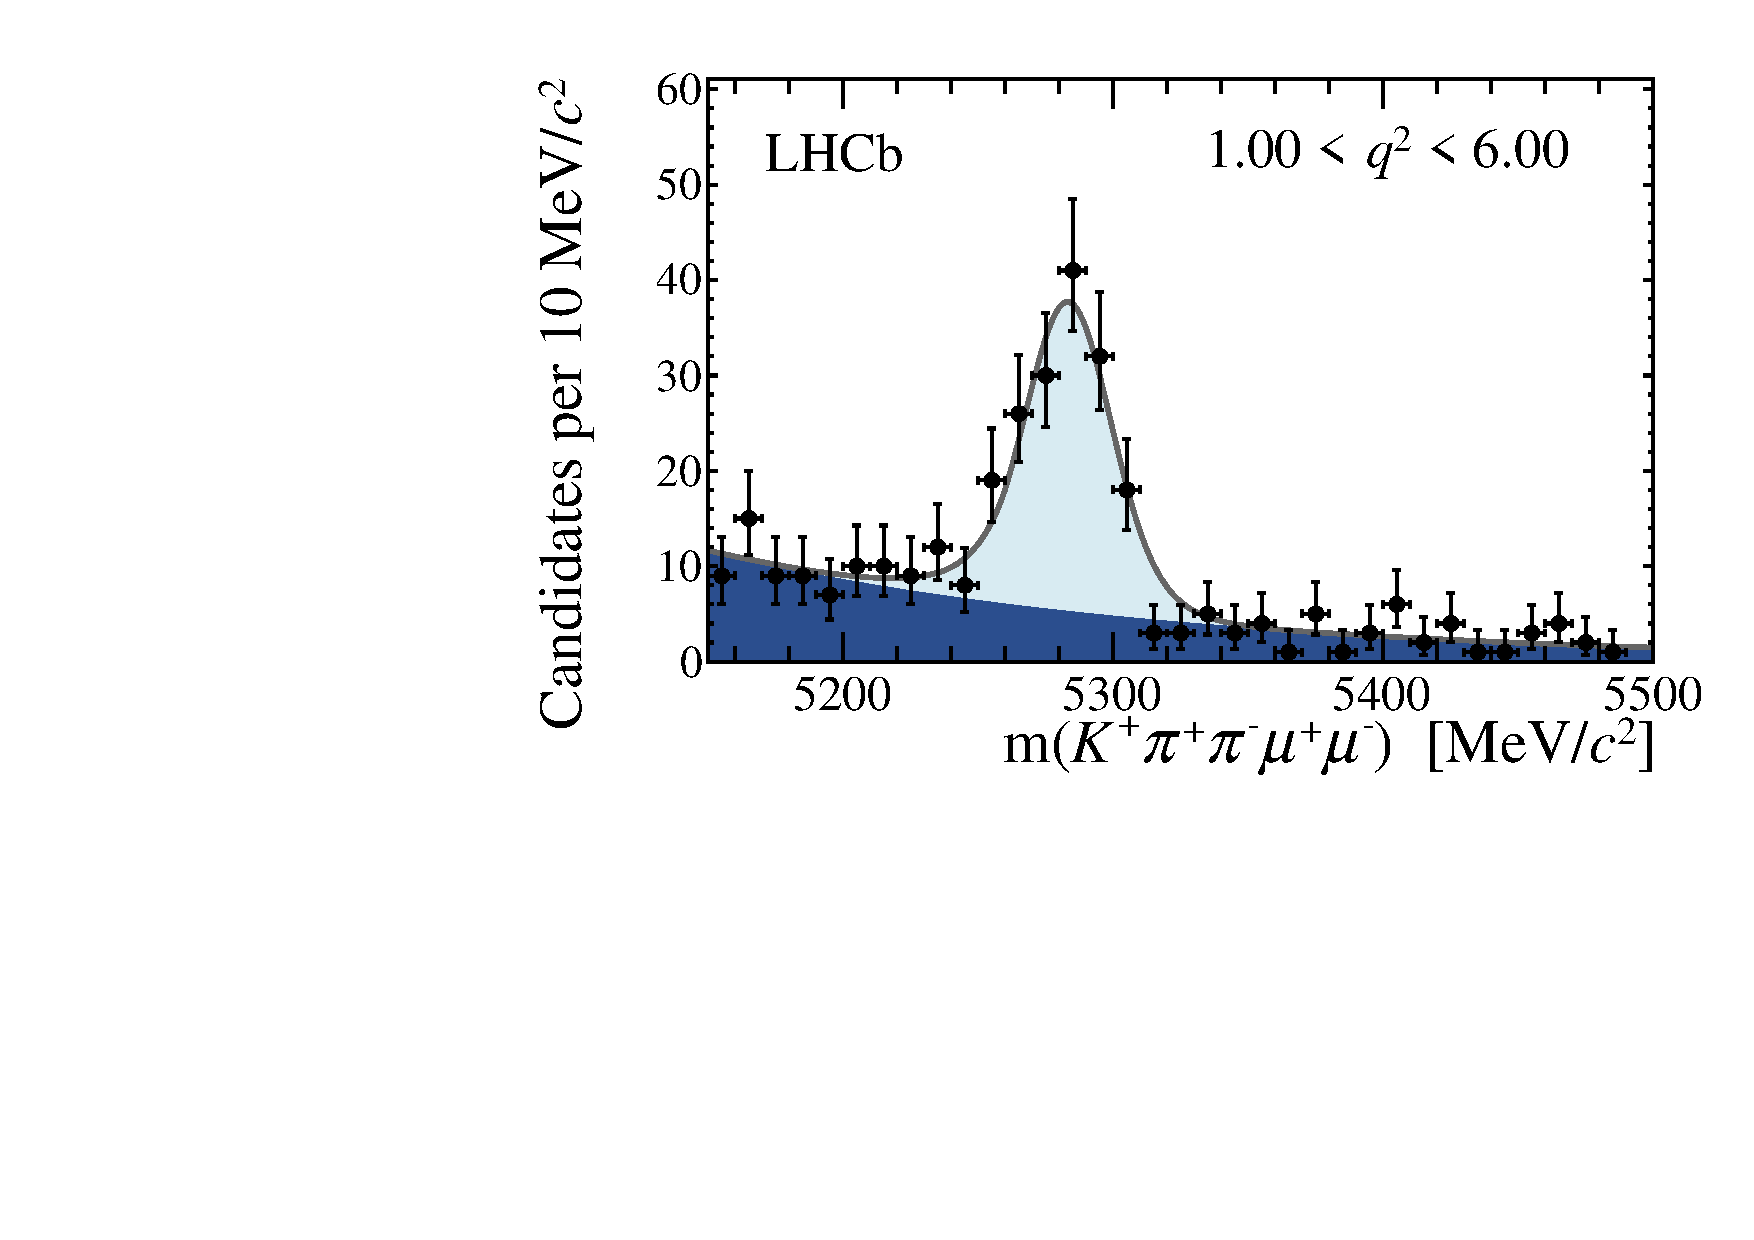
\includegraphics[width=0.48\textwidth]{q2_r1}
  %\end{center}
  %\caption{Plots for this section 1}
%\end{figure}
%
%
%\begin{figure}
  %\begin{center}
    %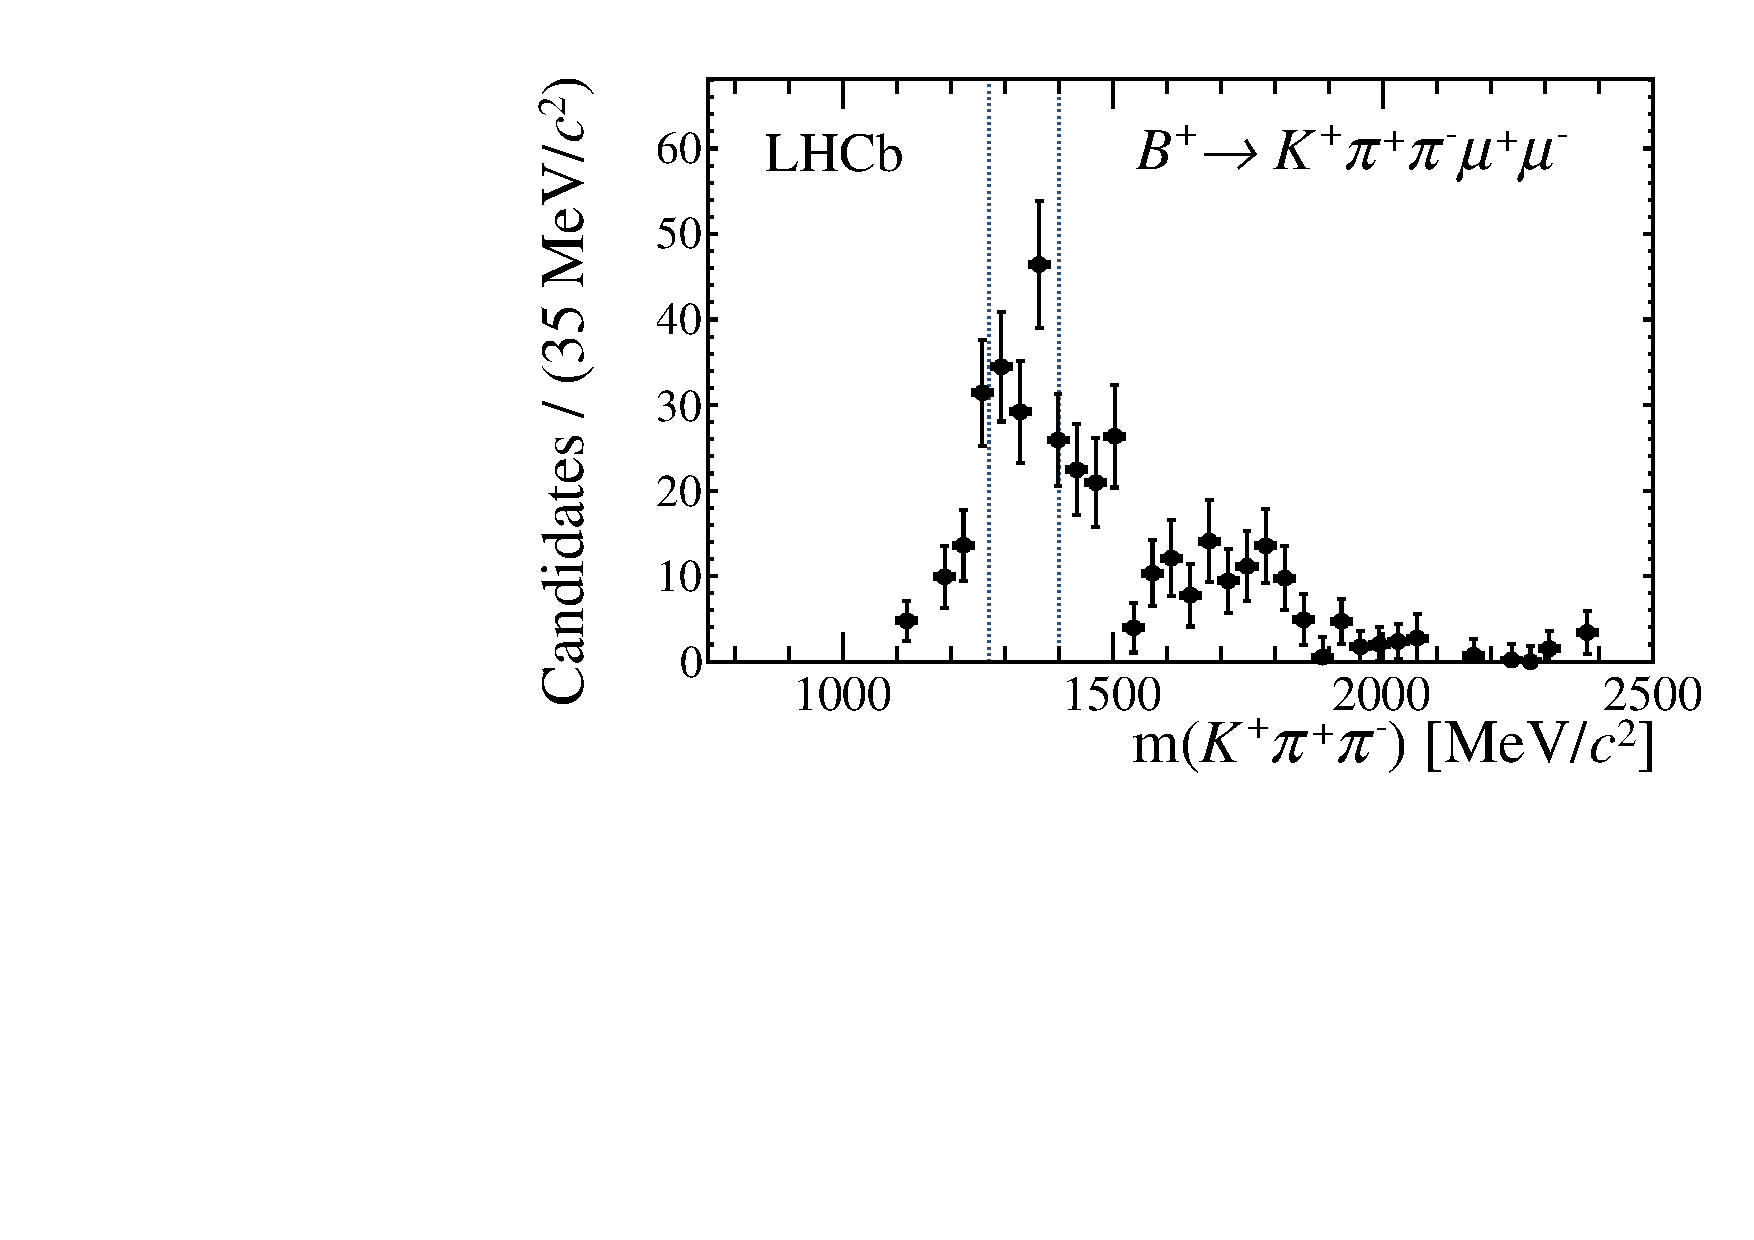
\includegraphics[width=0.48\textwidth]{kpipi_frommumu}
    %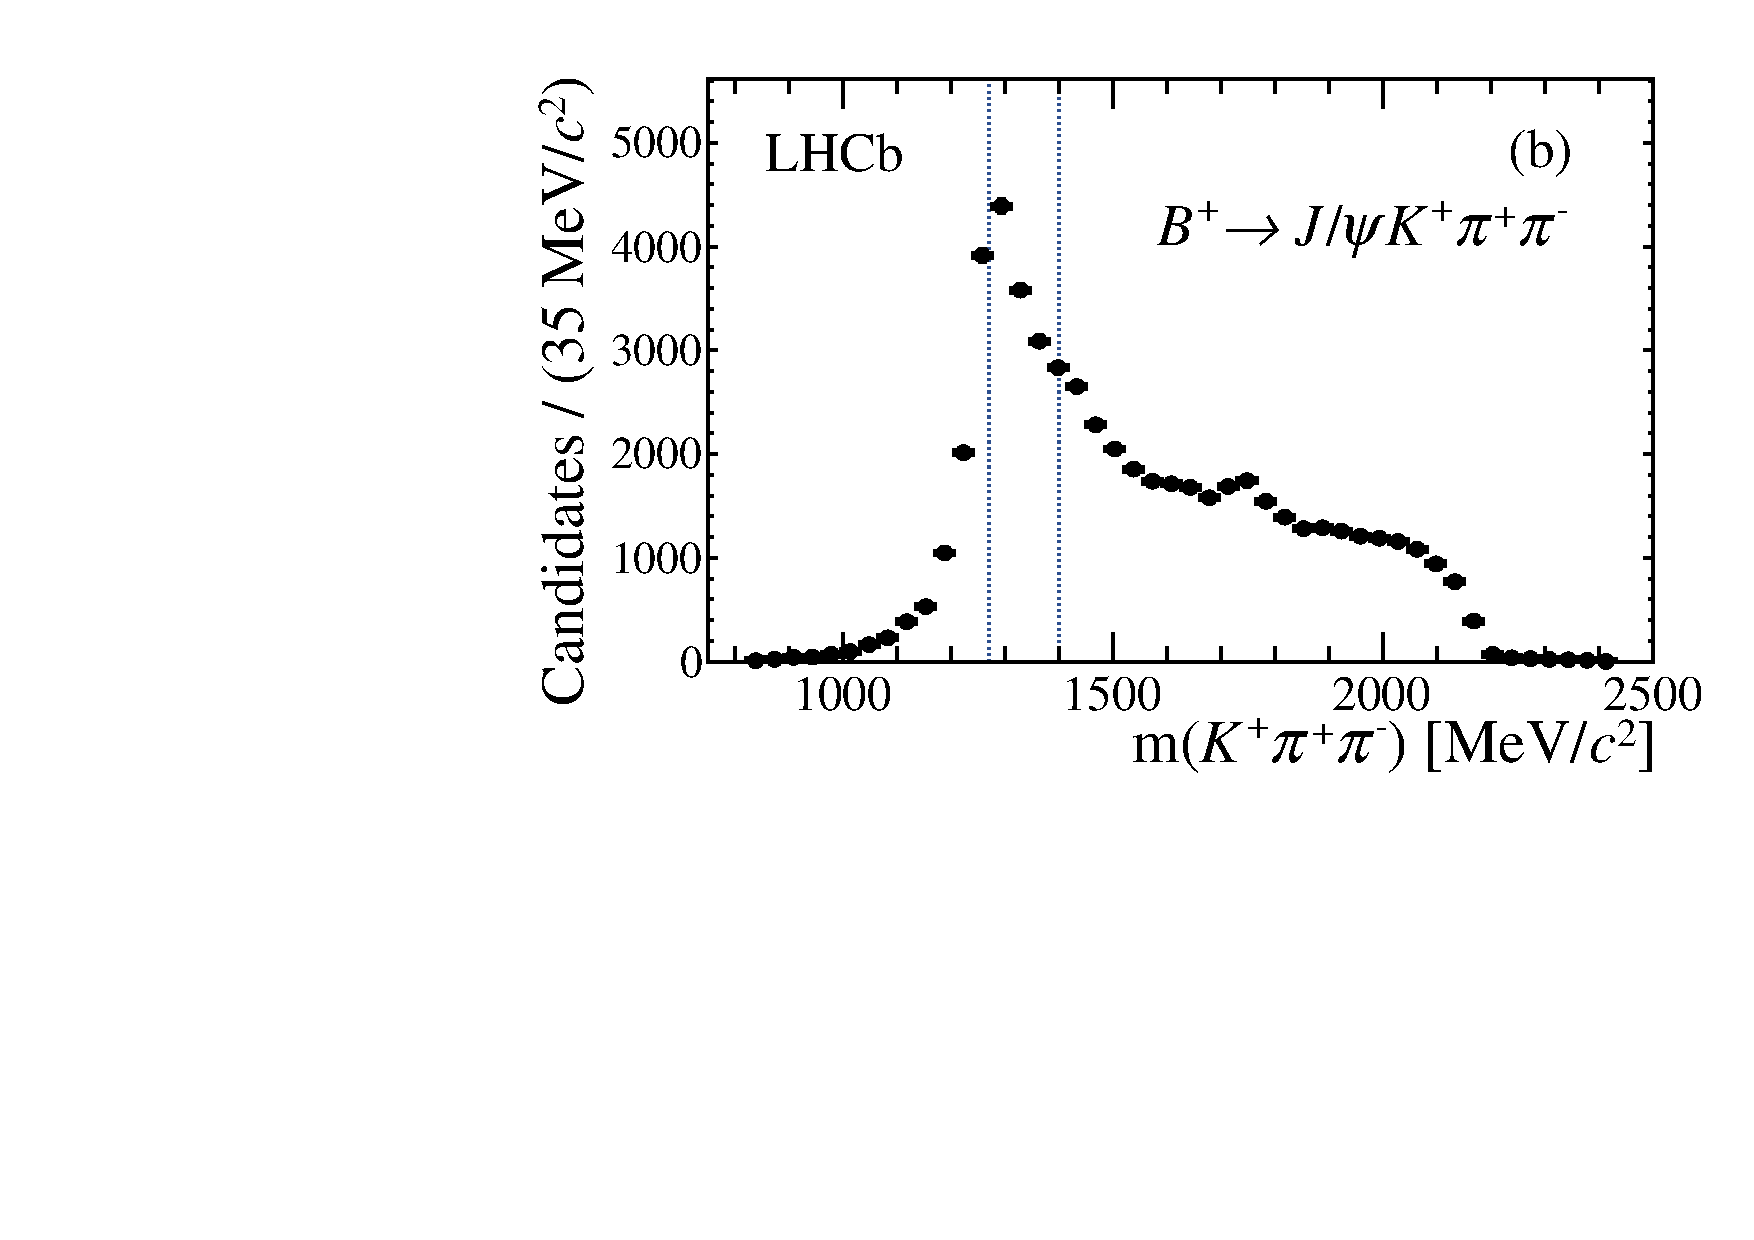
\includegraphics[width=0.48\textwidth]{kpipi_fromjpsi}
    %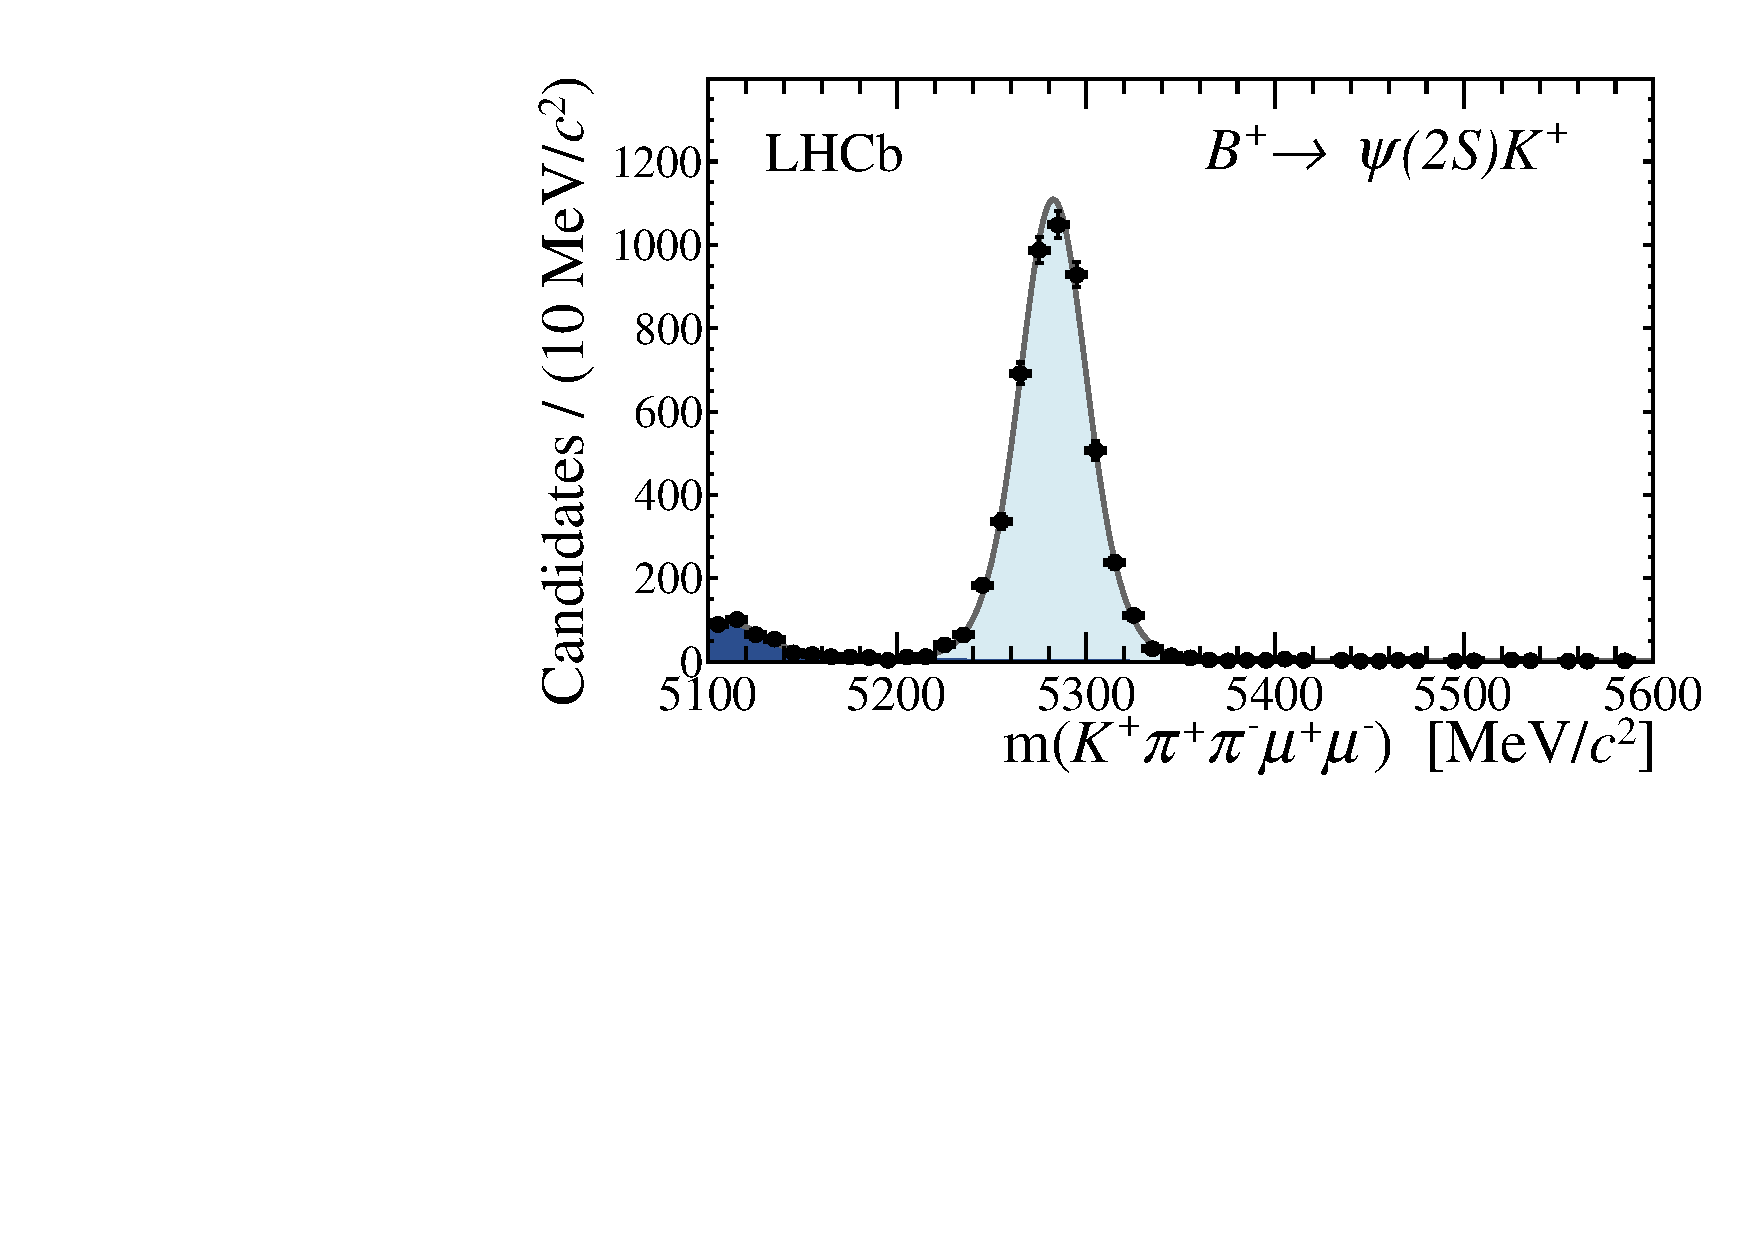
\includegraphics[width=0.48\textwidth]{b2psi2sk}
    %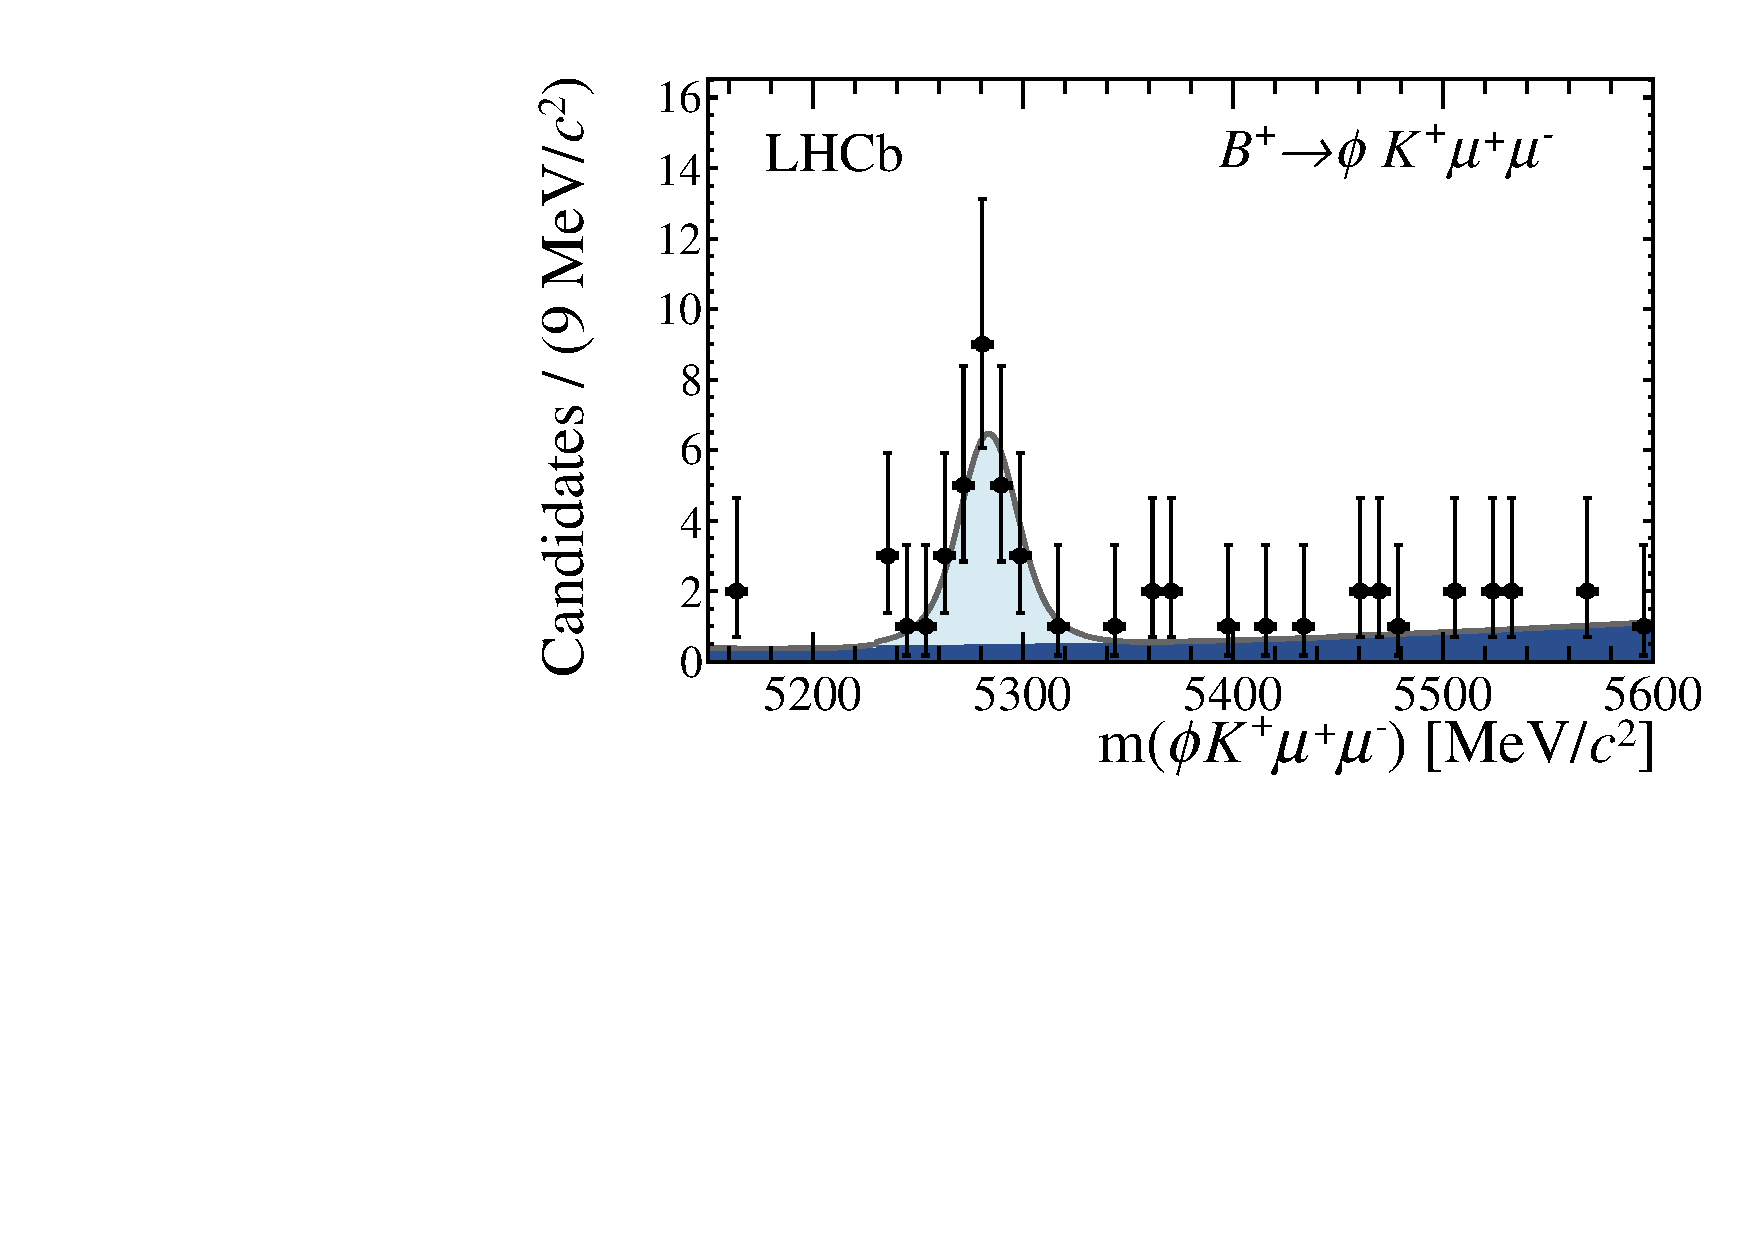
\includegraphics[width=0.48\textwidth]{b2phikmumu}
    %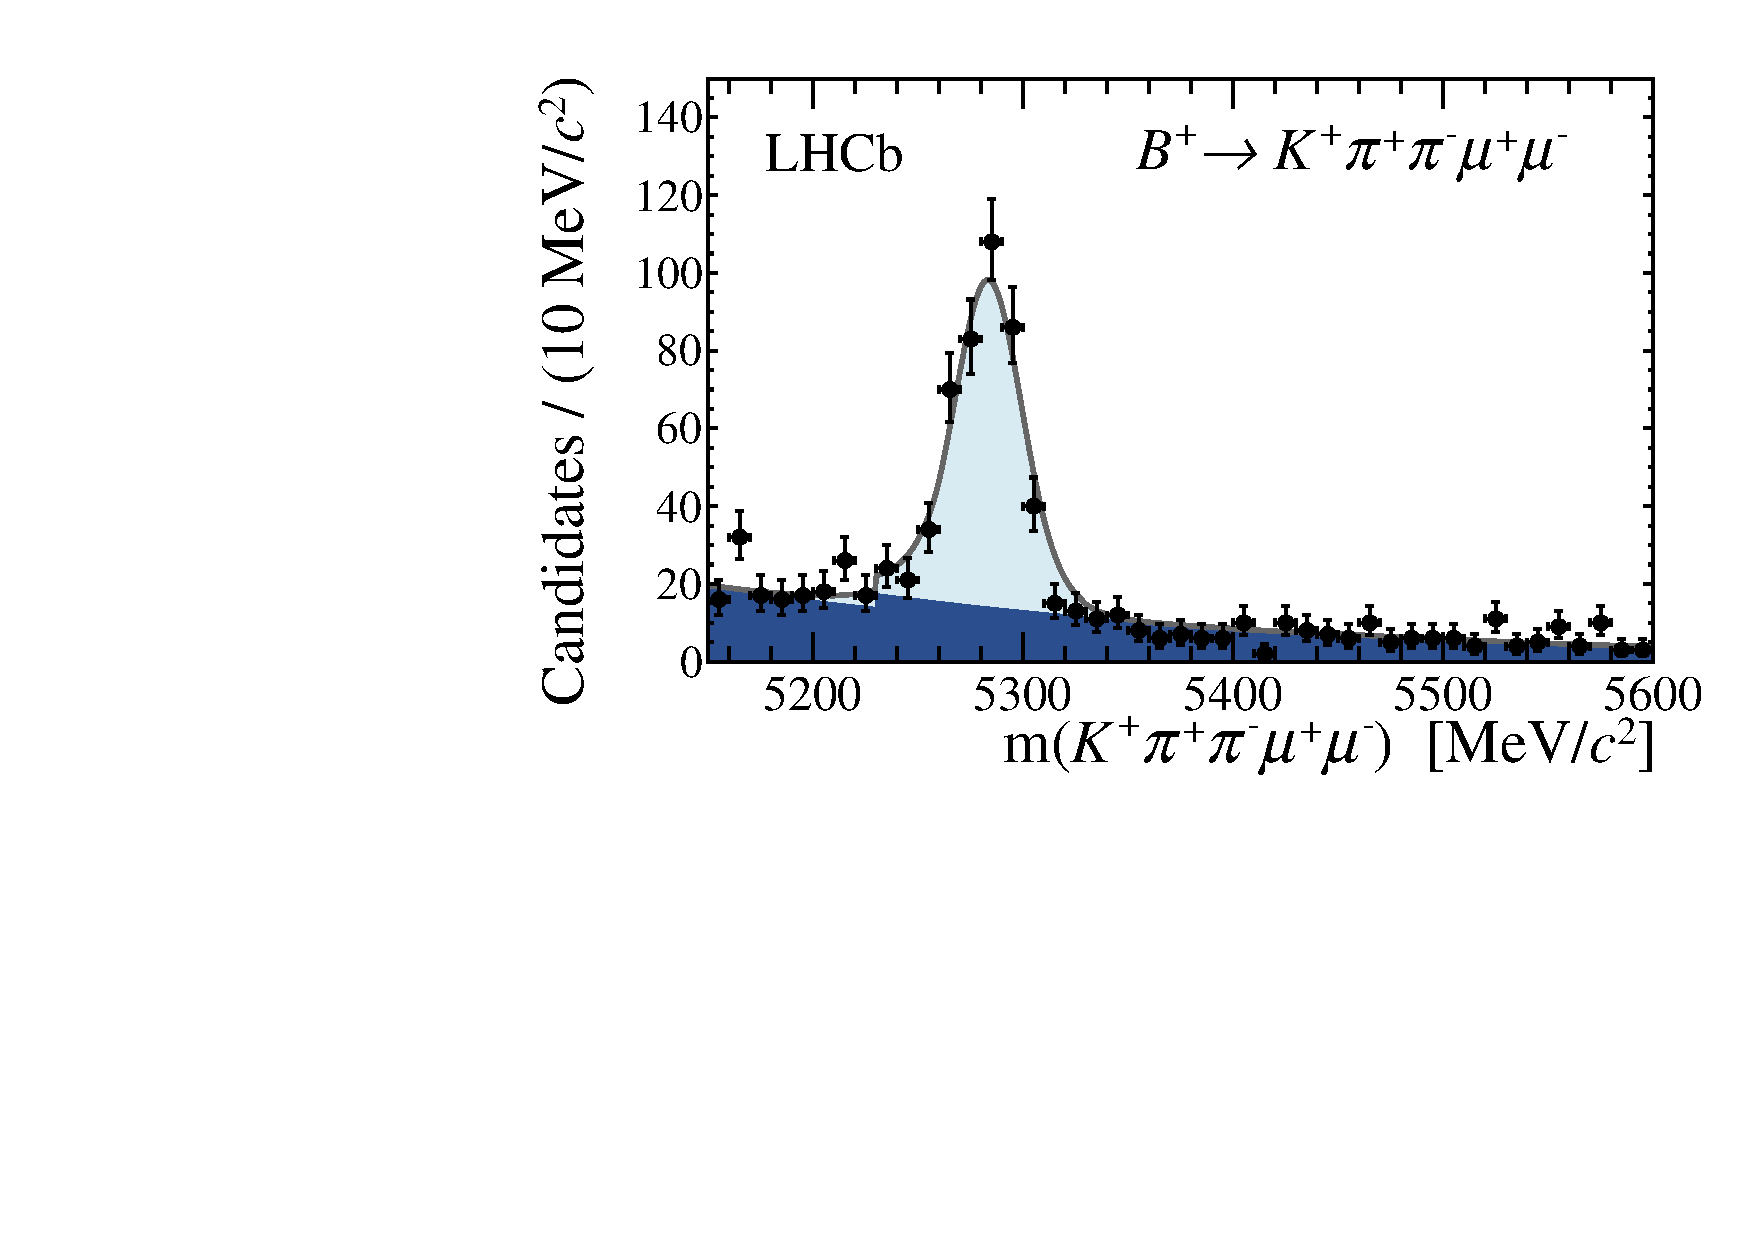
\includegraphics[width=0.48\textwidth]{b2kpipimumu}
    %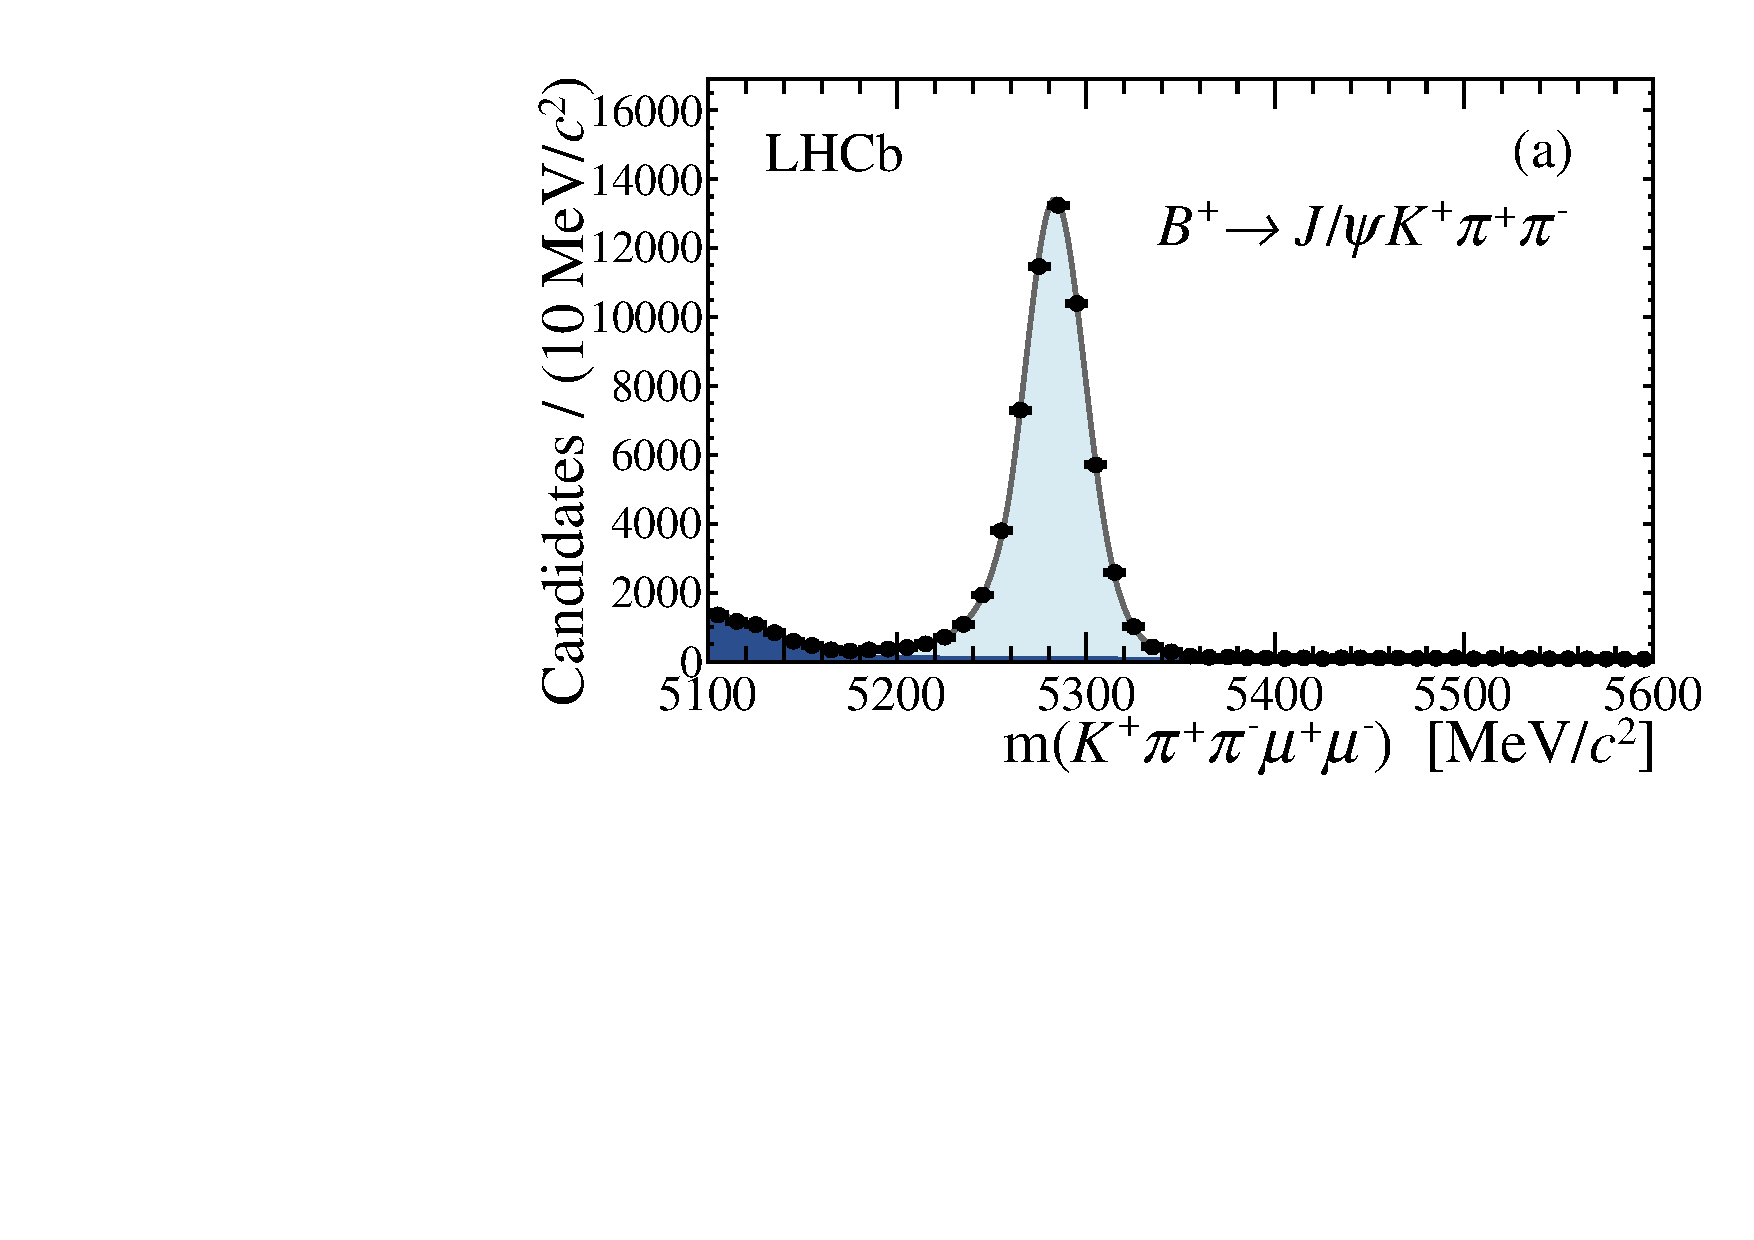
\includegraphics[width=0.48\textwidth]{b2kpipijpsi}
  %\end{center}
  %\caption{Plots for this section 2}
%\end{figure}
%
%

\cite{Alves:2008zz}
